\documentclass[12pt]{article}
\usepackage[utf8]{inputenc}
\usepackage{lmodern}
%\usepackage[brazilian]{babel} % Use this if you want PT-BR
\usepackage[T1]{fontenc}
\usepackage{natbib}
\usepackage[top=2cm, bottom=2cm, left = 2cm, right=2cm]{geometry}
\usepackage{amsmath}
\usepackage{amsthm}
\usepackage{amssymb}
\usepackage{bbm}
\usepackage{mathtools}
\usepackage{graphicx}
\usepackage{hyperref}
\hypersetup{
    colorlinks=true,
    linkcolor=blue,
    filecolor=blue,      
    urlcolor=blue,
    citecolor = blue
}
\usepackage{subfig}
\usepackage{cleveref}
\usepackage{enumitem}
\usepackage{booktabs}
\usepackage{longtable}
\usepackage{adjustbox}
\usepackage{natbib}
\usepackage{caption}
\linespread{1.3}

\newtheorem{assumption}{Assumption}
\newtheorem{claim}{Claim}

\newcommand{\bigCI}{\mathrel{\text{\scalebox{1.07}{$\perp\mkern-10mu\perp$}}}}

\title{Microeconomics Applied to Brazil \\ Second Exam}
\author{Luis Antonio F. Alvarez}
\date{December 2017}

\begin{document}

\maketitle

\section*{Question 1}

We introduce FGTS as a transfer $\delta \tau_\omega w_F $ the formal worker receives upon becoming unemployed. The benefit is paid immediately after a match in the formal sector is terminated. The flow of being employed in the formal sector thus becomes:

\begin{equation}
    r E_F = (1 - \tau_\omega) w_F - s_F (E_F - U) + s_F b + s_F \delta \tau_\omega w_F 
\end{equation}

Notice that FGTS transfers to workers effectively act as a reduction of $100 \times \delta s_F \tau_\omega$ pp in the labour tax rate paid by formal employees (the ``effective'' labour tax rate is now $(1 - \delta s_F)\tau_\omega$). The remaining equations which describe the model (equations (2) to (6), (8) to (10) in the paper and the free entry conditions)  remain unchanged. Substituting the corresponding flow equations in the Nash bargaining FOC, and using the free entry conditions, we get the following expression for the wage in the formal sector:

\begin{equation}
    w_F = \frac{1}{1 - (1 - \delta s_F)\tau_\omega} \left[\frac{\phi_F}{1-\phi_F}\frac{(r+s_F)}{q_F}rK_F +rU-s_Fb\right]
\end{equation}

The expression for the wage in the informal sector remains unchanged:

\begin{equation}
    w_I = \frac{\phi_I}{1-\phi_I} \frac{r + S_I}{q_I} r K_I + rU
\end{equation}

Following the same steps in \cite{Ulyssea2010}, we are left with the following set of equations, which characterise labour market equilibria:
\begin{align}
rU = \frac{\phi_F}{1-\phi_F}rK_F\theta_F + \frac{\phi_I}{1-\phi_I}rK_I\theta_I  \\
p_F = a \gamma^{\rho -1}(a \gamma^\rho  + (1-a)(1-\gamma)^\rho)^\frac{1-\rho}{\rho} \\
p_I = (1-a)(1-\gamma)^{\rho-1} (a \gamma^\rho + (1-a)(1-\gamma)^\rho )^\frac{1-\rho}{\rho}\\
p_F= \frac{(1+\tau_\pi)}{1 - (1 - \delta s_F)\tau_\omega}\left[\frac{\phi_F(r+s_F)}{(1-\phi_F)q_F}rK_F + rU-s_Fb\right] + (r + s_F + q_F)\frac{rK_F}{q_F} \\
p_I = \frac{(r+s_I)}{(1-\phi_I)q_I}rK_I + rU + rK_I \\
\gamma = f(\theta_F,\theta_I) = \frac{\lambda_F s_I}{\lambda_F s_I + \lambda_I s_F}\\
q_j(\theta_j) = \frac{\lambda_j (\theta_j)}{\theta_j}, \quad j\in\{I,F\}
\end{align}
where the last equality follows from $m_j(u, v_j)$ displaying constant returns to scale for $j = I, F$.

Note that the expression for the wage differential in our case is:

\begin{equation}
    w_F - w_I = \frac{1}{1 - (1 - \delta s_F)\tau_\omega} \left[\frac{\phi_F}{1-\phi_F}\frac{(r+s_F)}{q_F}rK_F +rU-s_Fb\right] - \frac{\phi_I}{1-\phi_I} \frac{r + S_I}{q_I} r K_I + rU
\end{equation}

The expression for total welfare does not change:
\begin{equation}
    W = (1 - u)[\gamma(p_F - rK_f) + (1-\gamma)(p_I - rK_I)] - u [\gamma \theta_F r K_F + (1-\gamma) \theta_I r K_I]
\end{equation}
\subsection*{General equilibrium analysis}
We now analyse the effects of varying the fraction of contributions returned to formal workers upon entering unemployment ($\delta$). Partial equilibrium analyses where we hold labour tightness constant are uninteresting in our case\footnote{It does not make much sense to vary $\delta$ while keeping labour market tightness constant -- in the same way as one would not, in a simple supply-and-demand competitive labour market analysis, change tax rates while holding aggregate employment constant.}. We thus follow a general equilibrium analysis. We use \cite{Ulyssea2010}'s benchmark parameter values  (Table 3 in his paper) to initialise the model. We then look at the equilibrium degree of informality ($1-\gamma$), wage differential ($\frac{w_F - w_I}{w_I}$) and social welfare ($W$) when varying $\delta$. Notice that $\delta = 0$ should yield similar results as the author's.

Python codes for this exercise can be found at my GitHub page\footnote{Link: \url{https://github.com/luisfantozzialvarez/exammicrobrazil/tree/master/Exam2MicroBrazil}.}. The resulting plots are displayed in \Cref{fig:gen_eq}. As one can see, increasing the proportion $\delta$ that is returned to formal workers upon entering unemployment decreases the degree of informality and increases welfare. This seems intuitive, as formal jobs become more attractive\footnote{The main chain of causation for the increase in formality goes somewhat as follows: when $\delta$ is raised, workers at the formal sector are willing to accept a smaller $w_F$ in the bargaining process, as they know that, in the future, they will receive higher transfers if the match is terminated. This increases the value of a vacancy in the formal sector, which leads to firms posting more formal jobs. The net equilibrium effect is an increase in the degree of formality. } (the ``effective'' labour tax rate, $(1 - \delta s_F)\tau_\omega$, decreases) and less income is pumped out of the economy in net terms. One also sees that the wage differential between sectors decreases. Indeed, when increasing $\delta$, the formal worker is willing to accept a lower wage $w_F$ in the bargain, as she knows she will receive a higher transfer in the future if her match is terminated. The equilibrium wage, $w_F$, decreases; but notice from the last plot that the ``effective'' wage rate in the formal sector, $(1 - (1 - \delta s_F)\tau_\omega)w_F$, actually increases. 

\begin{figure}
    \centering
     \caption{General equilibriuma analysis: varying $\delta$}
    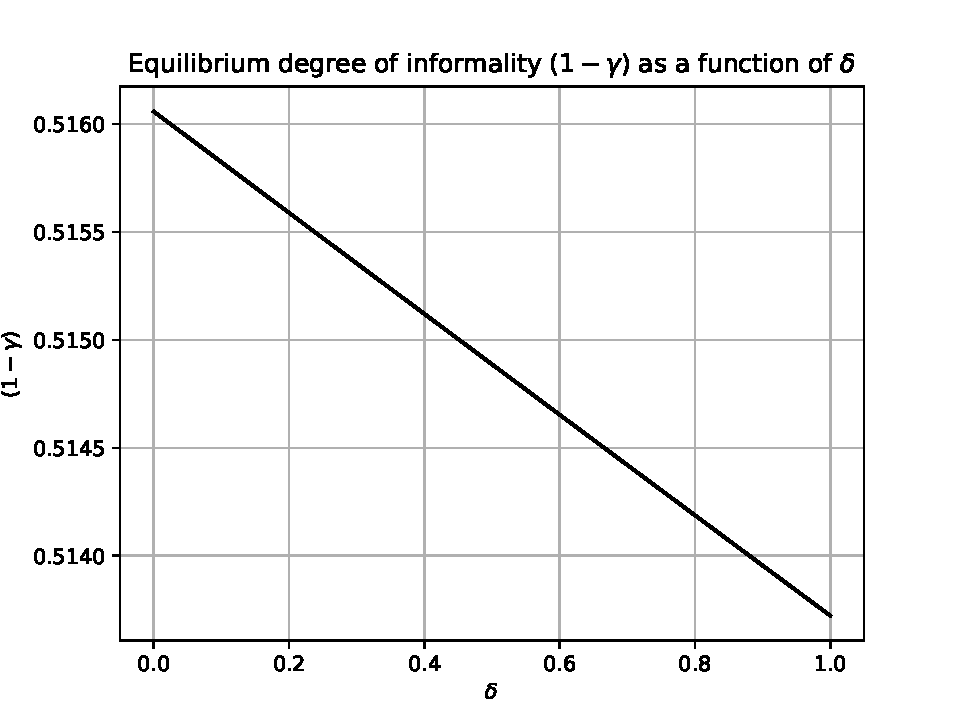
\includegraphics[scale = 0.9]{figures/informality.pdf}
    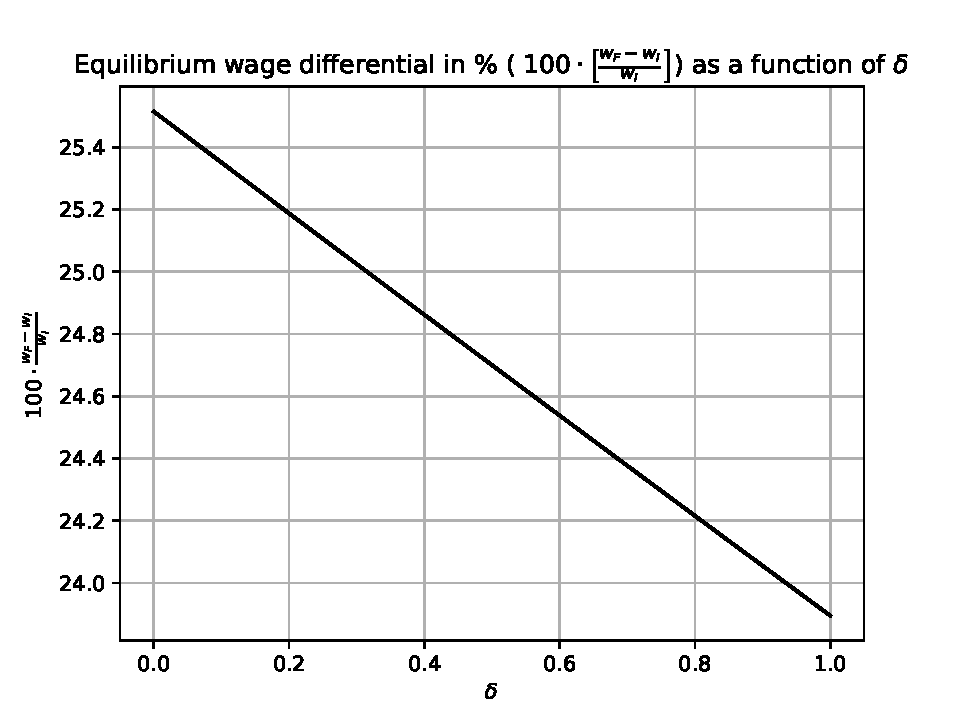
\includegraphics[scale = 0.9]{figures/wagegap.pdf}

    \label{fig:gen_eq}
\end{figure}

\begin{figure}\ContinuedFloat
    \centering
    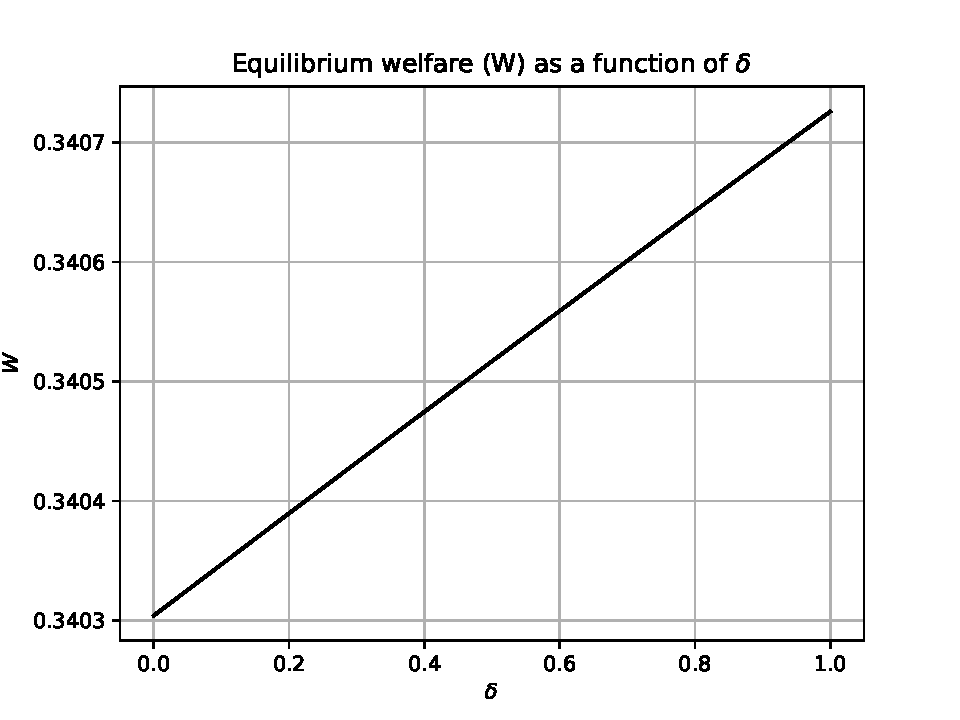
\includegraphics[scale = 0.9]{figures/welfare.pdf}
    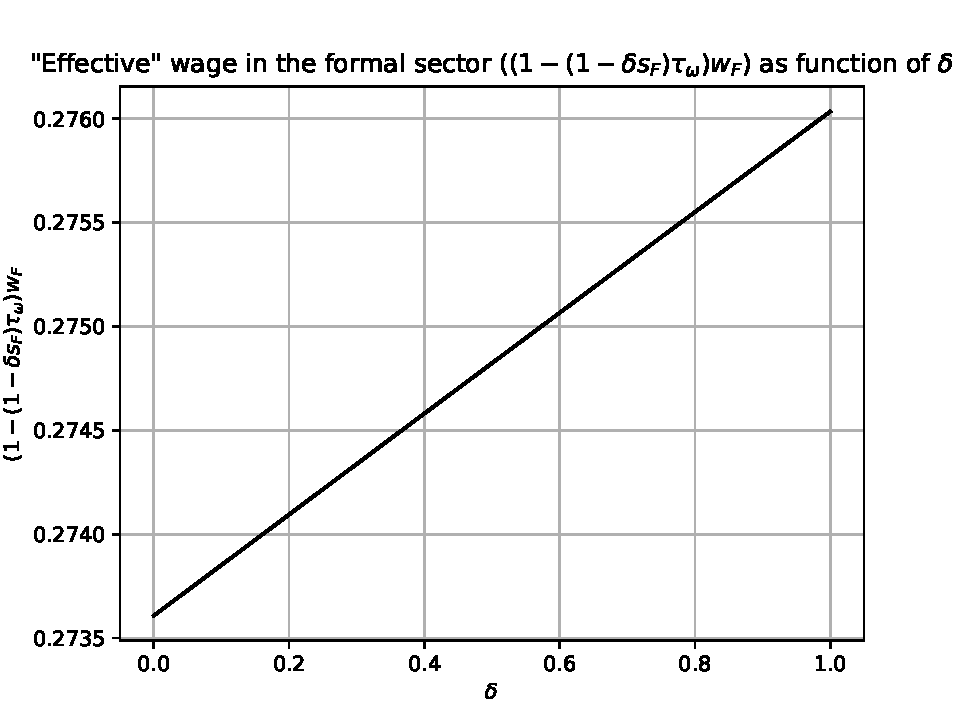
\includegraphics[scale = 0.9]{figures/effective.pdf}
\end{figure}



\bibliographystyle{chicago}
\bibliography{bib}
\end{document}


